%% LyX 2.3.1 created this file.  For more info, see http://www.lyx.org/.
%% Do not edit unless you really know what you are doing.
\documentclass[language=finnish]{utuftlabreport}
\setcounter{secnumdepth}{2}
\setcounter{tocdepth}{2}
\ifx\hypersetup\undefined
  \AtBeginDocument{%
    \hypersetup{unicode=true}
  }
\else
  \hypersetup{unicode=true}
\fi
\addbibresource{Bibliografia.bib}
\begin{document}
% Document template suitable for use as a latex master-file for lab
% reports in University of Turku Department of Future Technologies. 

% This template is synced with the gitlab template.
% Works with sharelatex / pdflatex / xelatex

% --
% --
% Relies on utuftlabreport.cls for the document class definitions.

% Traditionally the best places to learn (La)TeX are probably the manual
% pages for each package
%   http://www.ctan.org/ 
% and
%  http://www.ctan.org/tex-archive/info/lshort/english/lshort.pdf

% This version should be compatible with xelatex and biblatex
% which means that all source files can freely use normal UTF-8 text
% without resorting to "legacy hacks".
%
%
% The utuftlabreport.cls defines a new lab report class, which is based on
% the report class.

\publab{Tietotekniikka}

\pubcourse{Hajautetut ohj.järjestelmät ja pilvipalvelut}

\groupmembers{Mikko Mallikas (123456)}
\title{Harjoitustyö 1\\
{\large{}Laskennan nopeuttaminen säieohjelmoinnilla}}

\maketitle
\tableofcontents{}

\chapter{Johdanto}

Nykyään on tavallista, että muutaman euron arvoisista sulautetuista
järjestelmistä alkaen tietokoneet sisältävät useampia ns. suoritinytimiä
ja sitä kautta kyvyn laskea yhden sijaan useita laskutoimituksia samanaikaisesti.
Erilaiset laskentatehtävät rinnakkaistuvat eri tavalla, mutta laskennan
tehostamisen kannalta helpoin algoritmien kategoria on ns. helposti
rinnakkaistuvat ongelmat (\textit{embarrassingly parallel}). Nämä
algoritmit voidaan osittaa niin, että osat voidaan laskea täysin itsenäisesti
ilman kommunikointia osien välillä. Käytännössä tällaiset ongelmat
voidaan jakaa aluksi osaongelmiin, käynnistää kunkin osan suoritus
rinnakkain ja/tai peräkkäin ja odottaa, kunnes kaikki laskenta päättyy,
jonka jälkeen tulokset kootaan.

\section{Mandelbrot-fraktaali}

Tässä harjoitustyössä sovelletaan yhtä tällaista ongelmaa – ns. Mandelbrotin
fraktaalijoukon kuvan piirtämistä rinnakkaisesti. Kuvan piirtämisessä
keskeinen osa on ns. ydinfunktio (\textit{kernel}), joka saa syötteenä
kuvapisteen koordinaatit ja generoi iteratiivisella kompleksilukuaritmetiikalla
kuvapisteelle värin annetusta paletista. Jokaisen pisteen väriarvo
voidaan laskea toisista pisteistä riippumatta – laskennan perustaksi
riittää siis pelkkä pisteen koordinaatti. Säieohjelmoinnin tekniikoiden
vastuulle jää koordinoida korkean tason suoritus niin että kaikki
kuvan $leveys \times korkeus$ pistettä tulevat lasketuksi mahdollisimman
tehokkaasti.

\section{Säikeistystehtävät\label{sec:S=0000E4ikeistysteht=0000E4v=0000E4t}}

Tässä harjoitustyössä on seuraavat kolme ratkaistavaa säieohjelmoinnin
ongelmaa:
\begin{enumerate}
\item Ratkaistaan ongelma \textit{staattisella aikataulutuksella}, so. tilanne,
jossa kukin säie $p_1, ..., p_n$ saa tehtäväksi kiinteän määrän tehtäviä
$t_1, ..., t_m$. Kutakin tehtävää vastaa yhtäsuuri kuva-alue kokonaiskuvasta.
Esimerkki: $n=4$ ja $m=2$. Nyt jokainen prosessori saa kaksi tehtävää,
joista kumpikin vastaa $\frac{1}{n \times m} = \frac{1}{8}$ koko
kuvasta. Kuvan voi jakaa esim. allekkain kahdeksaan vaakasuoraan siivuun.
Kun säie on suorittanut tehtävänsä $t_1$, jatkaa se suoraan tehtävästä
$t_2$. Nyt jos jonkin muun säikeen tehtävä on vielä keskeneräinen,
näitä tehtäviä ei jaeta säikeiden välillä vaan nopeiten valmistuvat
jäävät odottamaan.
\item Ratkaistaan ongelma \textit{dynaamisella aikataulutuksella}, so. tilanne,
jossa kukin säie $p_1, ..., p_n$ saa tehtäväksi vaihtelevan määrän
tehtävistä $t_1, ..., t_m$. Kutakin tehtävää vastaa tässäkin yhtäsuuri
kuva-alue kokonaiskuvasta, mutta algoritmin ero syntyykin siinä, miten
tehtäviä jaetaan. Esimerkki: $n=4$ ja $m=64$. Nyt jokainen säie
saa tehtävän, joka vastaa $\frac{1}{m} = \frac{1}{64}$ koko kuvasta.
Kuvan voi jakaa esim. ''tiiliin'', niin että kokonaiskuva koostuu
$8 \times 8$ pienemmästä ruudusta, joiden kunkin koko on $\frac{leveys}{8} \times \frac{korkeus}{8}$.
Suoritettuaan tehtävänsä säie poimii jonosta uuden tekemättömän tehtävän,
kunnes kaikki tehtävät on laskettu.
\item Käyttöliittymän (piirretään uudelleen 50 ms välein) irrottaminen laskennasta:
\end{enumerate}
\begin{javacode}
class Ticker implements Scheduled {
  public int tickDuration() { return 50; }
  public void tick() {
      ...
      canvas.redraw();
      ...
  }
}
\end{javacode}
\begin{itemize}
\item[~] Nyt ongelma on, mikäli fraktaalin iteraatioiden maksimimäärää kasvattaa
tai ohjelmassa hiirellä navigoi työläästi laskettavaan kohtaan, laskenta
voi kestää yli 50 millisekuntia, jolloin keskeneräistä laskentaa voi
kumuloitua, minkä seurauksena koko käyttöliittymä voi ''halvaantua''.
Ongelmaan ratkaisuna on ns. työjono, joka on säieturvallinen samanaikainen
jonorakenne, johon yhteen päähän tallennetaan seuraava piirrettävä
kuva ja toisesta päästä luetaan käyttöliittymän esitettäväksi jonoon
kertynyt kuva. Ongelma on klassinen tuottaja–kuluttaja -ongelma samanaikaisuuden
kirjallisuudesta. Tässä lisähaasteina on
\item Käyttöliittymää saa JavaFX:ssä päivittää vain JavaFX:n käyttöliittymäsäikeellä
tai ohjelma kaatuu. JavaFX-säie tarjotaan automaattisesti ja kyseinen
säie kutsuu Ticker-luokan metodeita ja oletuksena sitä kautta koko
piirtoa alusta loppuun.
\item Toiseksi, kuvat vievät kohtalaisen paljon muistitilaa, joten työjono
ei voi olla mielivaltaisen suuri vaan jonon pituus kannattaa rajoittaa,
esim. sulavan toiminnan takaamiseksi 2–3 kuvaan (jonossa on tällöin
valmiina kuvia, mikäli laskenta tilapäisesti kestää yli 50 ms)
\item Jonosta kulutetaan kuvia pois tasaisella 50 ms nopeudella (+ piirto
JavaFX:llä kesti harj.työn laatijan koneella lähes vakioajan 1-2 ms),
joten jos tuottaja pystyy tuottamaan kuvan välillä nopeammin, tuottaminen
tulisi jäädyttää säietekniikoilla, kunnes jonoon mahtuu taas kuvia.
\item Toisaalta, kuluttaja ei saa vastaavalla tavalla jäädä odottamaan jonosta
kuvaa, mikäli seuraava näytettävää kuvaa ei ole, sillä tämä jäädyttäisi
käyttöliittymän kuten alkeellinen ratkaisu ilman työjonoa. Jos jono
on tyhjä, käyttöliittymän tulee jatkaa vanhan kuvan näyttämistä.
\end{itemize}

\section{Alustava toteutus}

Tehtävänannon pohjana käytettävä toteutus mallintaa Mandelbrot-fraktaalin
laskennan peräkkäisesti. Toteutus on tehty Java-kielellä ja hyödyntää
grafiikan esittämiseen modernia JavaFX-kirjastoa. Työssä sekä kytkös
JavaFX:ään että laskennan ydinfunktio (sekä muu työn tekoa helpottava
käyttöliittymä) tarjotaan valmiina. Työ vaatii siis aluksi jonkin
verran olemassaolevan koodin opiskelua (noin 900 riviä ml. kommentit),
mutta tässä on se hyöty, että työn varsinainen kurssin teorian kannalta
tärkeä toteutus on varsin pelkistetty ja ytimekäs.
\begin{enumerate}
\item Fraktaalin piirto lähtee liikkeelle matalimmalla tasolla luokista
\begin{enumerate}
\item MandelbrotKernel: yleinen rajapinta Mandelbrot-kuvapisteen laskemiseksi
\item MandelbrotSlowKernel: toteuttaa pisteen laskennan yksinkertaisella
skalaarimatematiikalla (double)
\item MandelbrotFastKernel: toteuttaa pisteen laskennan vektorimatematiikalla
(4:n mittainen double-taulukko\footnote{Java kutsuu laitteistotasolla NEON/SSE/AVX/AltiVec-käskyjä tässä yhteydessä.})
\end{enumerate}
\item Piirron seuraava luokkien abstraktiotaso hyödyntää Javan (8+) moniperintää
\begin{enumerate}
\item MandelbrotRenderer: yleinen kehys koko fraktaalin laskemiseksi
\item RendererBase: yleinen kehys koko fraktaalin laskemiseksi
\item MandelbrotSequentialRenderer: piirtää fraktaalin peräkkäisesti
\item MandelbrotSlowRenderer: piirtää fraktaalin peräkkäisesti MandelbrotSlowKernel:lla
\begin{enumerate}
\item SlowRenderer: yhdistää MandelbrotSlowRenderer:n laskentakoodiin
\end{enumerate}
\item MandelbrotFastRenderer: piirtää fraktaalin peräkkäisesti MandelbrotFastKernel:lla
\begin{enumerate}
\item FastRenderer: yhdistää MandelbrotFastRenderer:n laskentakoodiin
\end{enumerate}
\item RendererFactory: apuluokka, joka luo pyynnöstä em. piirtoluokkia
\end{enumerate}
\item Seuraavat luokat tulisi ryhmän toteuttaa tehtävänannon mukaisesti
\begin{enumerate}
\item MandelbrotStaticParallelRenderer: piirtää fraktaalin rinnakkaisesti
MandelbrotFastKernel:lla, hyödyntäen staattista aikataulutusta
\begin{enumerate}
\item StaticThreadRenderer: yhdistää MandelbrotStaticParallelRenderer:n
laskentakoodiin
\end{enumerate}
\item MandelbrotDynamicParallelRenderer: piirtää fraktaalin rinnakkaisesti
MandelbrotFastKernel:lla, hyödyntäen dynaamista aikataulutusta
\begin{enumerate}
\item DynThreadRenderer: yhdistää MandelbrotDynamicParallelRenderer:n laskentakoodiin
\end{enumerate}
\end{enumerate}
\end{enumerate}
Lisäksi käyttöliittymän irrottaminen asynkronisesti laskennan suorittamisesta
vaatii ylimääräistä koodia yhteen tai useampaan projektin luokkaan
(vihjeeksi luokat, joita ei tarvitse muokata, on merkitty luokkia
edeltäviin kommentteihin).

Katsotaan esimerkinomaisesti luokkaa MandelbrotKernel (sivuutetaan
rotaatio):

\begin{javacode}
interface MandelbrotKernel {
  int vectorSize();
  int getMaxIterations();
  int mandelbrot(double c_re, double c_im);
  int[] mandelbrot(double x, double y, double inc, double rot);
}
\end{javacode}
\begin{itemize}
\item Metodi vectorSize() palauttaa joko 1 (slow) tai 4 (fast).
\item getMaxIterations() kertoo piirtoon asetettujen iteraatioiden maksimimäärän.
\item mandelbrot(c\_re, c\_im): laskee fraktaalin väriarvon pisteessä (c\_re,
c\_im)
\item mandelbrot(x, y, inc, rot): laskee fraktaalin väriarvot pisteissä
(x, y), (x+inc, y), (x+2{*}inc, y), (x+3{*}inc, y)
\item Yleisesti, em. kategorioiden 2) ja 3) luokat huolehtivat näistä matalan
tason rutiineista eikä niistä tarvitse välittää (pl. se fakta, että
drawTile-jaon koordinaattirajojen pitää olla vektoriprosessoinnin
takia neljällä jaollisia!)
\end{itemize}
Katsotaan esimerkinomaisesti luokkaa MandelbrotSequentialRenderer:

\begin{javacode}
interface MandelbrotSequentialRenderer extends MandelbrotRenderer {
  default void drawSet(Viewport vp) {
    drawTile(0, 0, renderWidth(), renderHeight(), vp);
  }
}
\end{javacode}
\begin{itemize}
\item Metodi drawSet piirtää koko fraktaalin ja delegoi oletuksena työn
metodille drawTile. Vastaava metodi voi ryhmän toteutettavaksi jäävissä
luokissa käsittää rinnakkaisen strategian piirtää fraktaali.
\item Metodi drawTile (luokasta MandelbrotRenderer) laskee peräkkäisesti,
iteratiivisesti, rivi ja sarake kerrallaan alueen (0,0) – (renderWidth(),
renderHeight()) kaikki kuvapisteet. Tätä metodia (ja sitä matalamman
tason asioita) ei tarvitse muokata.
\end{itemize}
Lisäksi työn kannalta on olennainen seuraava luokkajoukko, joka käsittää
fraktaalin säilömiseen tarkoitetun ''piirtopinnan'':
\begin{itemize}
\item PixelRenderer: rajapinta, joka kytkee piirron konkreettiin piirtopintaan.
\item FXPixelRenderer: edellisen konkreetti toteutus JavaFX:n piirtorutiineille.
\item MandelbrotCanvas: yleinen piirtopinnan ja näkymän säilövä apuluokka.
\item FXMandelbrotCanvas: edellisen konkreetti toteutus JavaFX:n piirtorutiineille.
\item Ticker: kytkee FXMandelbrotCanvas:n JavaFX:n ikkunaan ja tapahtumankäsittelyyn.
\end{itemize}

\section{Käytännön toteutus}

\subsection{Työkalut}
\begin{itemize}
\item Työn tekemistä varten, asenna seuraavat työkalut seuraavassa järjestyksessä:
\end{itemize}
\begin{enumerate}
\item Java: \href{https://www.oracle.com/technetwork/java/javase/downloads/index.html}{oracle.com/technetwork/java/javase/downloads/}
\item Git: \href{https://git-scm.com/downloads}{git-scm.com/downloads}
\item SBT: \href{https://www.scala-sbt.org/}{www.scala-sbt.org/}
\item IDEA: \href{https://www.jetbrains.com/idea/download/}{www.jetbrains.com/idea/download/}
\begin{enumerate}
\item IDEA:n asetusten kautta (File -> Configure -> Plugins + Install Jetbrains
plugin) Scala-plugin.
\item Valinnaisesti pluginit: Gitlab projects, Junit ja JavaFX.
\item Säädä myös File -> Settings -> Build, execution, deployment -> Build
tools -> sbt -> Project level settings -> {[}x{]} use auto-import
\end{enumerate}
\item JavaFX
\begin{itemize}
\item Java 10/11 (suositus)
\begin{itemize}
\item lataa käyttöjärjestelmäsi SDK-paketti (zip) osoitteesta\\
\url{https://gluonhq.com/products/javafx/}
\item tee kotikansioon hakemisto openjfx
\item pura zip sinne
\item tämä vaihe valinnainen, jos käytät SBT:tä
\end{itemize}
\item JavaFX 8
\begin{itemize}
\item Windows/Mac: Oracle JDK (tulee mukana)
\item Linux: OpenJFX (pitää asentaa erikseen paketinhallinnasta)
\end{itemize}
\end{itemize}
\end{enumerate}

\subsection{Konfigurointi}
\begin{itemize}
\item Ympäristömuuttujat
\begin{itemize}
\item {\small{}Windows: Select Start -> Computer -> System Properties ->
Advanced system settings -> Environment Variables -> System variables
-> PATH. ...}{\small\par}
\item Mac: ohje vaihtelee valitettavasti versioittain
\item Linux: editoi \textasciitilde /.profile tai \textasciitilde /.bashrc
\item Aetukset päivittyvät kun sisäänkirjautuu uudestaan!
\end{itemize}
\item Ympäristömuuttuja\texttt{\textbf{\footnotesize{} JAVAFX\_HOME (ei
välttämätön)}}{\footnotesize\par}
\begin{itemize}
\item viittaa yllä valittuun javafx-kansion juureen
\item esim. /home/minä/openjfx
\end{itemize}
\item Ympäristömuuttuja\texttt{\textbf{\footnotesize{} PATH}}{\footnotesize\par}
\begin{itemize}
\item Testaa että komentoriviltä voi suorittaa käskyt: git, sbt, java, \textbf{javac}
(Oracle jostain syystä unohtanut jossain Java-versiossa sisällyttää
JDK:n javac:n PATH:iin)
\item Jos jokin työkalu ei toimi, lisää kyseisen työkalun binäärien hakemisto
PATHiin ;-eroteltuna (Linux/Mac :-eroteltuna).
\end{itemize}
\end{itemize}

\subsection{Projektin haku}
\begin{enumerate}
\item Lataa git-ohjelmalla projekti \url{TODO} \begin{nocode}
$ git clone TODO
$ cd TODO
\end{nocode}
\item tai gitlab-sivun pilvikuvakkeen takaa (jos et hallitse gitiä)
\item tai IDEA:lla (Check out from Version Control -> Git)
\begin{itemize}
\item Erikseen ladatun proj. voi importata myöhemminkin
\item SBT integroituna IDEA:n sisällä – ei tarvita komentoriviä
\item Java-versio valitaan projektia luotaessa. Voi vaihtaa myöh. Suositus:
11
\end{itemize}
\end{enumerate}
\begin{itemize}
\item Komentoriviltä projektin pitäisi käynnistyä käskyllä:
\end{itemize}
\begin{nocode}
$ sbt run
\end{nocode}

\chapter{Tehtävän kuvaus}

Toteuta luvun \ref{sec:S=0000E4ikeistysteht=0000E4v=0000E4t} kolme
säikeistystehtävää:

\section{Ratkaisu \textit{staattisella aikataulutuksella}}
\begin{itemize}
\item Jaa kuva yhtäsuuriin vaakasuoriin siivuihin ja laske ne rinnakkain.
\item Toteuta laskenta Thread/Runnable-luokkia käyttäen
\item Selvitä kokeellisesti ohjelman käyttöliittymän ja/tai benchmark-rutiinien
avulla konekokoonpanollesi optimaalinen määrä siivuja ja säikeitä.
\item Mikäli koneesi ei sisällä moniydinprosessoria (ts. > 8v vanha), säikeiden
käyttö ei ole järkevää tehtävässä alunperinkään, mutta voit lisätä
piirtorutiinin yhteyteen joka säikeelle Thread.sleep(5)-viiveen, jolloin
tehtävä on jälleen mielekäs.
\item Vinkki: tehtävä ei vaadi juurikaan koodin uudelleenjärjestelyä
\end{itemize}

\section{Ratkaisu\textit{ dynaamisella aikataulutuksella}}
\begin{itemize}
\item Jaa kuva yhtäsuuriin ''tiiliin'' laske ne rinnakkain.
\item Toteuta laskenta joko Thread/Runnable-luokkia käyttäen tai käytä apuna
Javan java.util.concurrent-luokkia
\item Selvitä kokeellisesti ohjelman käyttöliittymän ja/tai benchmark-rutiinien
avulla konekokoonpanollesi optimaalinen määrä tiiliä ja säikeitä.
\item Mikäli koneesi ei sisällä moniydinprosessoria (ts. > 8v vanha), säikeiden
käyttö ei ole järkevää tehtävässä alunperinkään, mutta voit lisätä
piirtorutiinin yhteyteen joka säikeelle Thread.sleep(5)-viiveen, jolloin
tehtävä on jälleen mielekäs.
\item Vinkki: tehtävä ei vaadi juurikaan koodin uudelleenjärjestelyä
\end{itemize}

\section{Käyttöliittymän irrottaminen laskennasta asynkronisesti}
\begin{itemize}
\item Toteuta piirron irrottaminen käyttöliittymäsäikeestä
\item Toteutuksessa kannattaa käyttää työmäärän vähentämiseksi vähintään
Javan tarjoamaa pinoluokkaa ja/tai java.util.concurrent-luokkia.
\item Totea asynkronisuuden toiminta lisäämällä laskennan kuormaa Detail++
-napista ja etsimällä kuvasta laskennallisesti vaativa kohta. Alkup.
toteutus jumiutuu pahasti. Ratkaisun tulisi pystyä vastaamaan käyttäjän
klikkailuun laskennan hidastumisesta huolimatta.
\item Vinkki: tehtävä vaatii koodin uudelleenjärjestelyä usean kuvan jonottamiseen
\item Mikäli koneesi sisältää vähän RAM-muistia, kytke päälle swap/page
file, pienennä koodista JavaFX-ikkunan kokoa ja/tai rajaa jonon pituus
2 kuvaan.
\item JavaFX:n ikkunan koko säädetään MandelbrotApp-luokan rivillä:
\end{itemize}
\begin{javacode}
  primaryStage.setScene(new Scene(
    root, screen.getWidth() * 2 / 3, screen.getHeight() * 2 / 3
  ));
\end{javacode}

\printbibliography


\appchapter{Liitedokumentti}

Mandelbrotin fraktaali perustuu kompleksilukufunktioon $x_{n+1} = x_{n}^2 + c$,
jossa x ja c ovat kompleksilukuja. C on vakio ja x:lle annetaan alkuarvoksi
$x_0 = (0, 0)$, tällöin yhtälöstä saadaan $x1 = c$ ja edelleen $x_2 = x_{1}^2 + c$.
Iterointia jatketaan kunnes x:n itseisarvo ylittää arvon 2. Jos $c$:n
itseisarvo on lähellä nollaa, niin x ei milloinkaan saavuta arvoa
2. Tätä vastaa fraktaalin kuvaajan keskellä oleva musta alue. Jos
$c$:n itseisarvo on suuri, esim 2, niin heti ensimmäinen iteraatio
saa x:n ylittämän arvon 2. Tätä vastaa kuvan reunoilla olevat tummimmat
alueet. Tällä välillä on epämääräisen muotoinen alue, jossa tarvittavien
iteraatiokierrosten määrä on vaikeasti ennustettavissa. Kuvassa kukin
piste vastaa yhtä $c$:n arvoa ja kyseisen pisteen väri kertoo tarvittujen
iterointikierrosten lukumäärän kyseisellä $c$:n arvolla. 

\begin{figure}
\begin{centering}
\vspace{-2cm}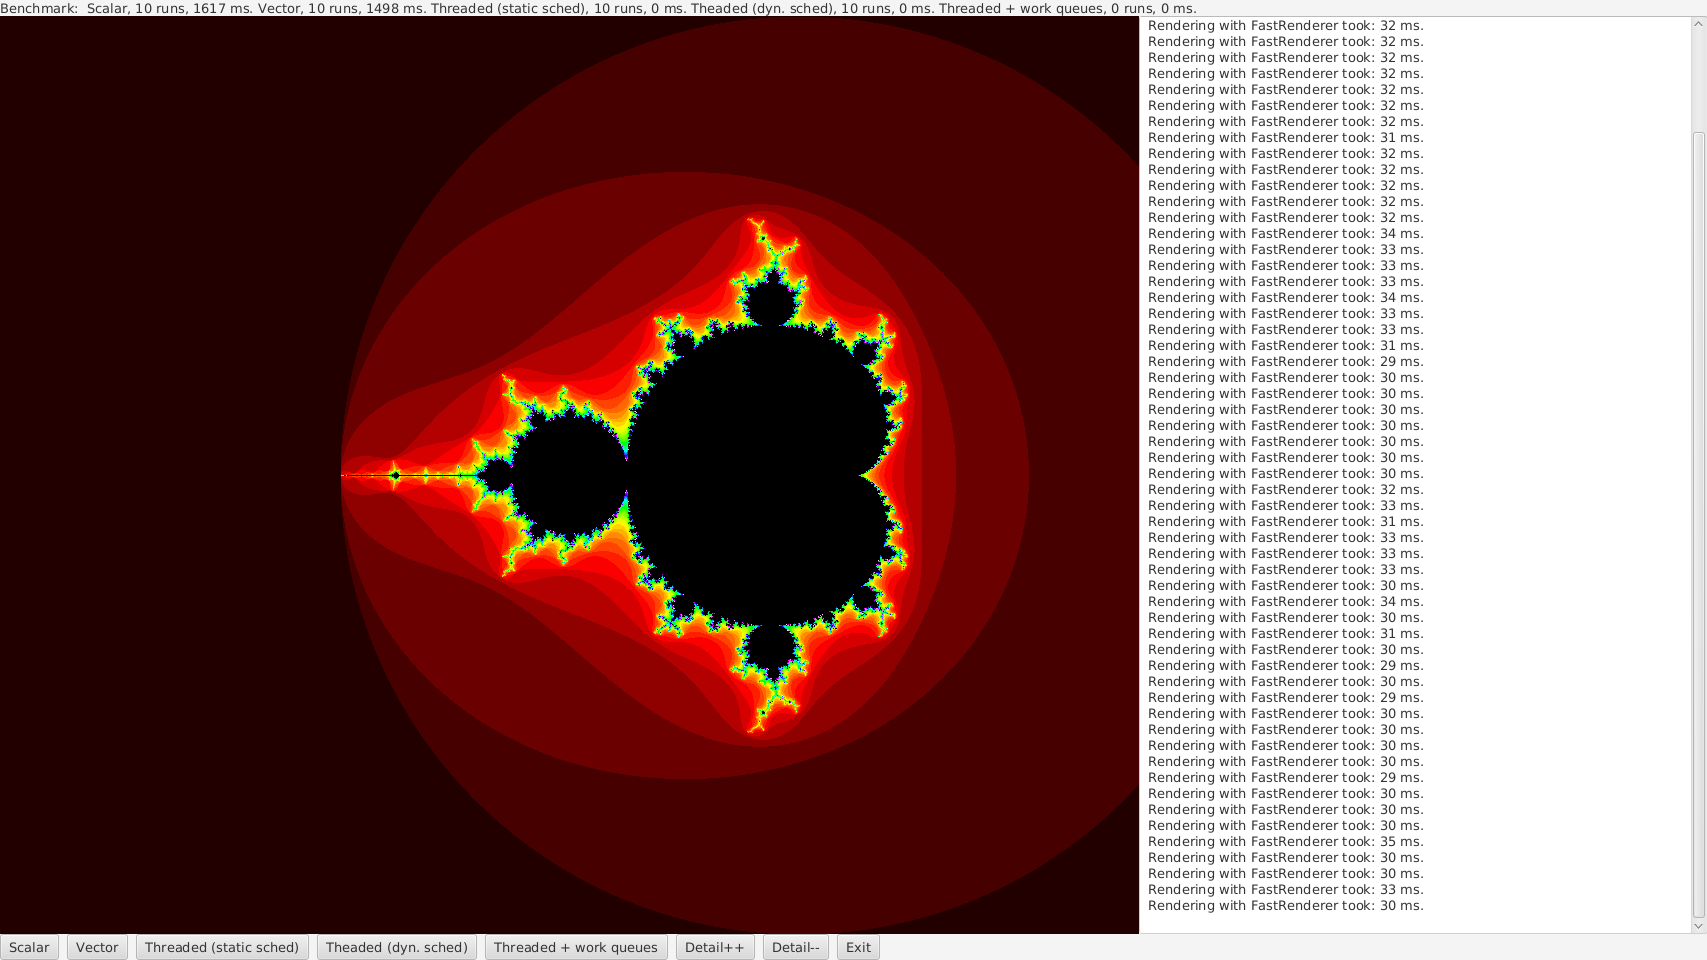
\includegraphics[width=0.9\textwidth]{kuvat/fexplorer}\vspace{-0.4cm}
\par\end{centering}
\caption{Mandelbrot-fraktaali työn ohjelmarungolla piirrettynä.}
\end{figure}

\end{document}
